\chapter{Podstawy teoretyczne} \label{chap:teoria}
W tym rozdziale zostaną omówione podstawowe pojęcia związane z tematem pracy. Pierwsze dwa podrozdziały skupiają się na opisie czym w ogóle jest aplikacja internetowa, oraz opisują jedno z najpopularniejszych podejść do budowania aplikacji internetowej, SPA. W kolejnych podrozdziałach zostały opisane technologie, które są porównywane w dalszej części pracy.
\section{Aplikacja internetowa}
Aplikacja internetowa jest czymś więcej niż zwykłą stroną internetową. Z definicji jest to aplikacja typu klient-serwer, w której klient jest uruchamiany przy pomocy przeglądarki internetowej. Oprogramowanie klienta jest pobierane na komputer klienta podczas wizyty na odpowiedniej stronie internetowej, przy użyciu standardowych procedur, takich jak HTTP. Aktualizacje oprogramowania klienta mogą odbywać się za każdym razem, gdy odwiedzana jest strona internetowa. W czasie trwania sesji przeglądarka internetowa interpretuje i wyświetla strony, oraz działa jako uniwersalny klient dla dowolnej aplikacji internetowej.
\begin{figure}[h]
	\centering
	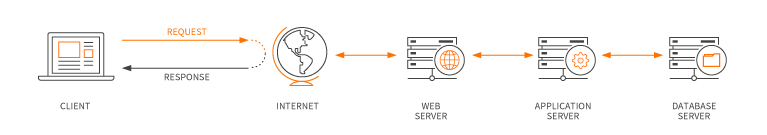
\includegraphics[width=\textwidth]{images/how_web_application_works}
	\caption{Podstawowy schemat działania aplikacji internetowej \cite{MaxCdnWebApp}}
\end{figure}
%\subsection{Krótki rys historyczny}
\section{SPA}Skrót SPA pochodzi od \textit{Single-page Application}. Jest to aplikacja internetowa działająca wewnątrz przeglądarki, która podczas użytkowania strony nie wymaga odświeżania strony. W tym podejściu, cały niezbędny kod źródłowy --- HTML, JavaScript i CSS --- jest pobierany przy pojedyńczym załadowaniu strony, lub odpowiednie zasoby są ładowane dynamicznie i dodawane do strony jedynie wtedy, kiedy jest to potrzebne. Idea jaka stoi za takim rozwiązaniem, to przede wszystkim lepszy, bardziej naturalny user expierience. Użytkownik po wejściu na stronę, nie musi przy każdej interakcji oczekiwać na ponowne załadowanie się strony, czy też jej odświeżanie.


\begin{figure}[!h]
	\centering
	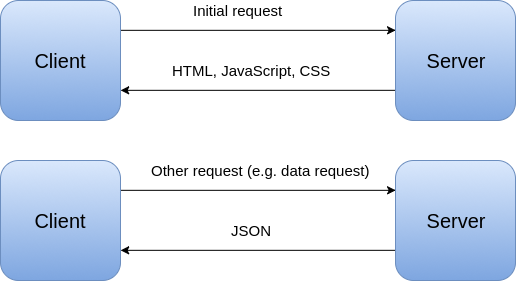
\includegraphics[width=0.6\textwidth]{images/spa}
	\caption{Podstawowy cykl życia SPA}
\end{figure}

Choć koncept SPA zaczął być częściej używany po spopularyzowaniu AJAX'a\footnote{Asynchronous JavaScript And XML}, to tak naprawdę dopiero od kilku lat jest on powszechnie wykorzystywany podczas budowania aplikacji internetowych. Serwisy takie jak Gmail, Google Maps, Twitter czy GitHub są właśnie aplikacjami typu single-page application. Także większość najpopularniejszych bibliotek JavaScript'owych umożliwiają implementację aplikacji internetowej zgodnie z zasadami SPA.
\subsection{Zalety}
\begin{itemize}
	\item Szybkość działania -- większość zasobów jest ładowana tylko raz podczas cyklu życia aplikacji, jedynymi informacjami, które są wymieniane z serwerem cały czas, są dane
	\item Brak ciągłego przeładowywania strony
	\item Znacznie prostszy proces wdrożenia aplikacji -- jedyne co jest potrzebne to statyczny serwer serwujący minimalnie 3 pliki -- pojedynczą stronę HTML, oraz 2 pakiety: jeden zawierający wszystkie style, drugi skupiający w sobie cały kod JavaScriptu
	\item Odciążenie strony serwerowej -- serwer, zamiast generować za każdym razem pełny kod strony, transmituje jedynie potrzebne w danej chwili dane
\end{itemize}
\subsection{Wady}
\begin{itemize}
	\item Powolne początkowe uruchomienie strony -- wymaga ono załadowania frameworku, oraz przynajmniej części aplikacji, która później już nie jest ponownie ściągana.
	\item Ze względu na zależność SPA od JavaScriptu, bardzo łatwo o pojawienie się wycieków pamięci pomiędzy długimi okresami czasu między przeładowaniami strony
\end{itemize}

\section{JavaScript}
JavaScript jest to wysokopoziomowy, słabo typowany, wieloparadgymatowy, skryptowy i interpretowany język programowania stworzony w 1995 roku przez Brendana Eicha dla firmy Netscape.  W roku 1997 organizacja Ecma International wydała na podstawie JavaScriptu standard języka skryptowego nazwany ECMAScript, na którym bazowanych jest większość silników JavaScript'owych.

JavaScript jest jedną z trzech głównych technologii wykorzystywanych przy tworzeniu treści związanych z siecią internetową. Obecnie 94,9\% spośród 10 milionów najbardziej popularnych stron internetowych wykorzystuje JavaScript (stan na grudzień 2017 \cite{JSUsage}).

\section{React.js}
React jest biblioteką języka JavaScript, wykorzystywaną do tworzenia graficznych interfejsów użytkownika. Pozwala ona na tworzenie rozbudowanych aplikacji internetowych, które używają danych i~mogą zmieniać swoją zawartość w czasie bez ponownego ładowania strony. Biblioteka została stworzona przez jednego z programistów Facebooka, Jordana Walke, który zainspirował się rozszerzeniem języka PHP, XHP, także stworzonym przez Facebooka. Pierwsze wersje biblioteki zostały użyte w 2011 roku na stronie aktualności Facebooka, a od 2012 roku jest ona wykorzystywana w~serwisie Instagram. Od 2013 roku React stał się wolnym oprogramowaniem, co spowodowało nagły wzrost jego popularności, a także umożliwiło społeczności  pomoc w rozwoju oprogramowania.

Ze względu na ogromny wpływ rynku urządzeń mobilnych, Facebook ogłosił w 2015 roku bibliotekę React Native, pozwalającą na korzystanie z architektury Reacta podczas budowania aplikacji mobilnych. To co wyróżniało tę bibliotekę od dotychczasowych sposobów tworzenia mobilnego oprogramowania, to brak konieczności powielania funkcjonalności dla każdej platformy z osobna. React Native pozwalał na wykorzystanie tego samego kodu źródłowego zarówno w aplikacji dla systemu Android jak i iOS.

Obecnie React jest jedną z najpopularniejszych bibliotek służących do tworzenia aplikacji internetowych. Jest wykorzystywany w ogromnej ilości znanych serwisów takich jak Facebook, Instagram, Spotify, Netflix czy eBay. 
\section{Redux}
Redux jest biblioteką języka JavaScript o otwartym kodzie źródłowym zaprojektowaną do zarządzania stanem aplikacji. Została stworzona w 2015 roku przez Dana Abramova. Działanie Reduxa może być opisane przez trzy zasady \cite{reduxDocs}:
\begin{enumerate}
	\item Istnieje jedno źródło prawdy -- stan całej aplikacji jest przechowywany w pojedyńczym obiekcie, który przechowuje całe drzewo stanu aplikacji.
	\item Stan służy tylko do odczytu -- jedynym sposobem na zmianę stanu jest wysłanie akcji -- obiektu opisującego co się stało, zwykle zawierającego typ akcji, oraz ewentualne dane, które mają wpływ na zmianę stanu.
	\item Zmiany stanu są dokonywane przy użyciu czystych funkcji -- aby określić, w jaki sposób drzewo stanu jest modyfikowane przez akcje, tworzy się funkcje zwane \textit{reducerami}, przyjmujące poprzedni stan i akcję jako argumenty, a zwracające nowy stan.
\end{enumerate}
\begin{figure}[h]
	\centering
	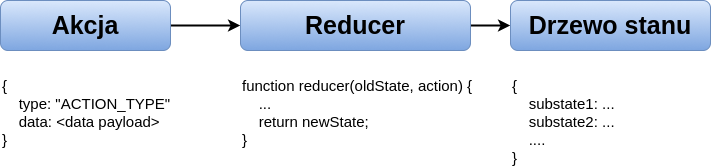
\includegraphics[width=0.9\textwidth]{images/redux_flow}
	\caption{Schemat działania Reduxa}
\end{figure}

\section{Elm}
Elm jest funcyjnym językiem programowania kompilowanym do JavaScriptu. Język został stworzony w 2012 roku przez Evana Czaplickiego, w ramach jego pracy dyplomowej. Na dalszy rozwój języka pozwoliła firma Prezi, która w 2013 roku zatrudniła twórcę języka. W 2016 roku Czaplicki zmienił firmę na NoRedInk i postanowił stworzyć organizację non-profit --- Elm Software Foundation --- której celem ma być promowanie, ochrona i rozwój języka Elm, oraz wszelka pomoc społeczności programistów tworzących oprogramowanie w Elmie \cite{newAdventures}.

Evan Czaplicki twierdzi, że jego język może konkurować z projektami takimi jak React, jako narzędzie do tworzenia aplikacji internetowych. Język kładzie bardzo duży nacisk na prostotę, łatwość użycia i jakość narzędzi \cite{elmGuide}.